\section{The Semantic Language Server}%
\label{sec:semantic_lsp}

During the development of the Semantic Language Server (SLS), we adhered to state-of-the-art implementation practices to ensure modularity, scalability, and maintainability\cite{10.1145/3550355.3552452,10.1145/3563834.3567537,10.1145/3550355.3552452,Bour_2018}.
Unlike traditional architectures, SLS leverages an entity component system (ECS), which offers greater separation of concerns compared to the widely recognized \textit{Layered Architecture}\cite{10.1145/3550355.3552452}.

\todo{Add information about Resources}
An ECS is a software design pattern that organizes a program into four key elements: Entities, Components, Systems, and Resources. 
In SLS, entities represent documents that are composed of various components. 
Components store data associated with the entity, such as the document's contents, file location, or derived RDF triples. 
Systems are functions designed to process specific components and are grouped into schedules to achieve distinct tasks. 
For example, the \textit{Parse} schedule includes systems responsible for tokenization, parsing, and triple extraction.
Semantic languages integrate seamlessly by introducing their systems into these predefined schedules to provide language-specific functionality.

As noted by Bour et al., “No spec, no tests” highlights the challenge of developing test suites for user-facing applications like language servers, where specifications can be open to interpretation\cite{Bour_2018}. 
To address this, SLS implements shared systems for common functionality, ensuring consistency and reducing redundancy across various semantic web languages.
By adopting this approach, SLS delivers uniform features, while maintaining flexibility for language-specific extensions.

SLS is implemented in Rust and leverages Bevy’s Entity Component System (ECS) to maintain a highly modular and efficient architecture.
Features are typically added in two steps:
  first, extracting the necessary data from RDF triples and attaching it to relevant entities; 
  second, using this data to implement language server functionalities such as diagnostics or autocompletion.

Bevy ECS facilitates this process by allowing the creation of isolated components and systems, enabling new features to be developed without impacting existing functionality.
This modularity ensures that only the minimal required data is extracted for each task, avoiding the complexity and overhead of constructing a complete digital twin of the dataset.

For example, to implement autocompletion based on defined classes, two small systems are added:
  one to extract information about defined classes and their descriptions,
  and another to incorporate this information into autocompletion requests. 
Similarly, adding a feature to display type hierarchies would involve creating a system to extract data specific to the rdfs:subclassOf relation, without interfering with other systems.
This approach allows for scalable and focused development of language server features.


\subsection{Language Server schedules}

This section details the systems implemented within each schedule of the Semantic Language Server (SLS).
Some systems are designed primarily to generate components, which are then utilized by other systems, potentially across different schedules.
This decoupled design ensures flexibility and modularity. 
If a system expects a component that is not present for a given entity, the system simply skips that entity.
This behavior supports asynchronous execution of systems, allowing for independent processing and reducing bottlenecks in the language server’s operation.

\subsubsection{Parse}

\begin{figure}[tb]
 \centering
 \makebox[\textwidth]{%
    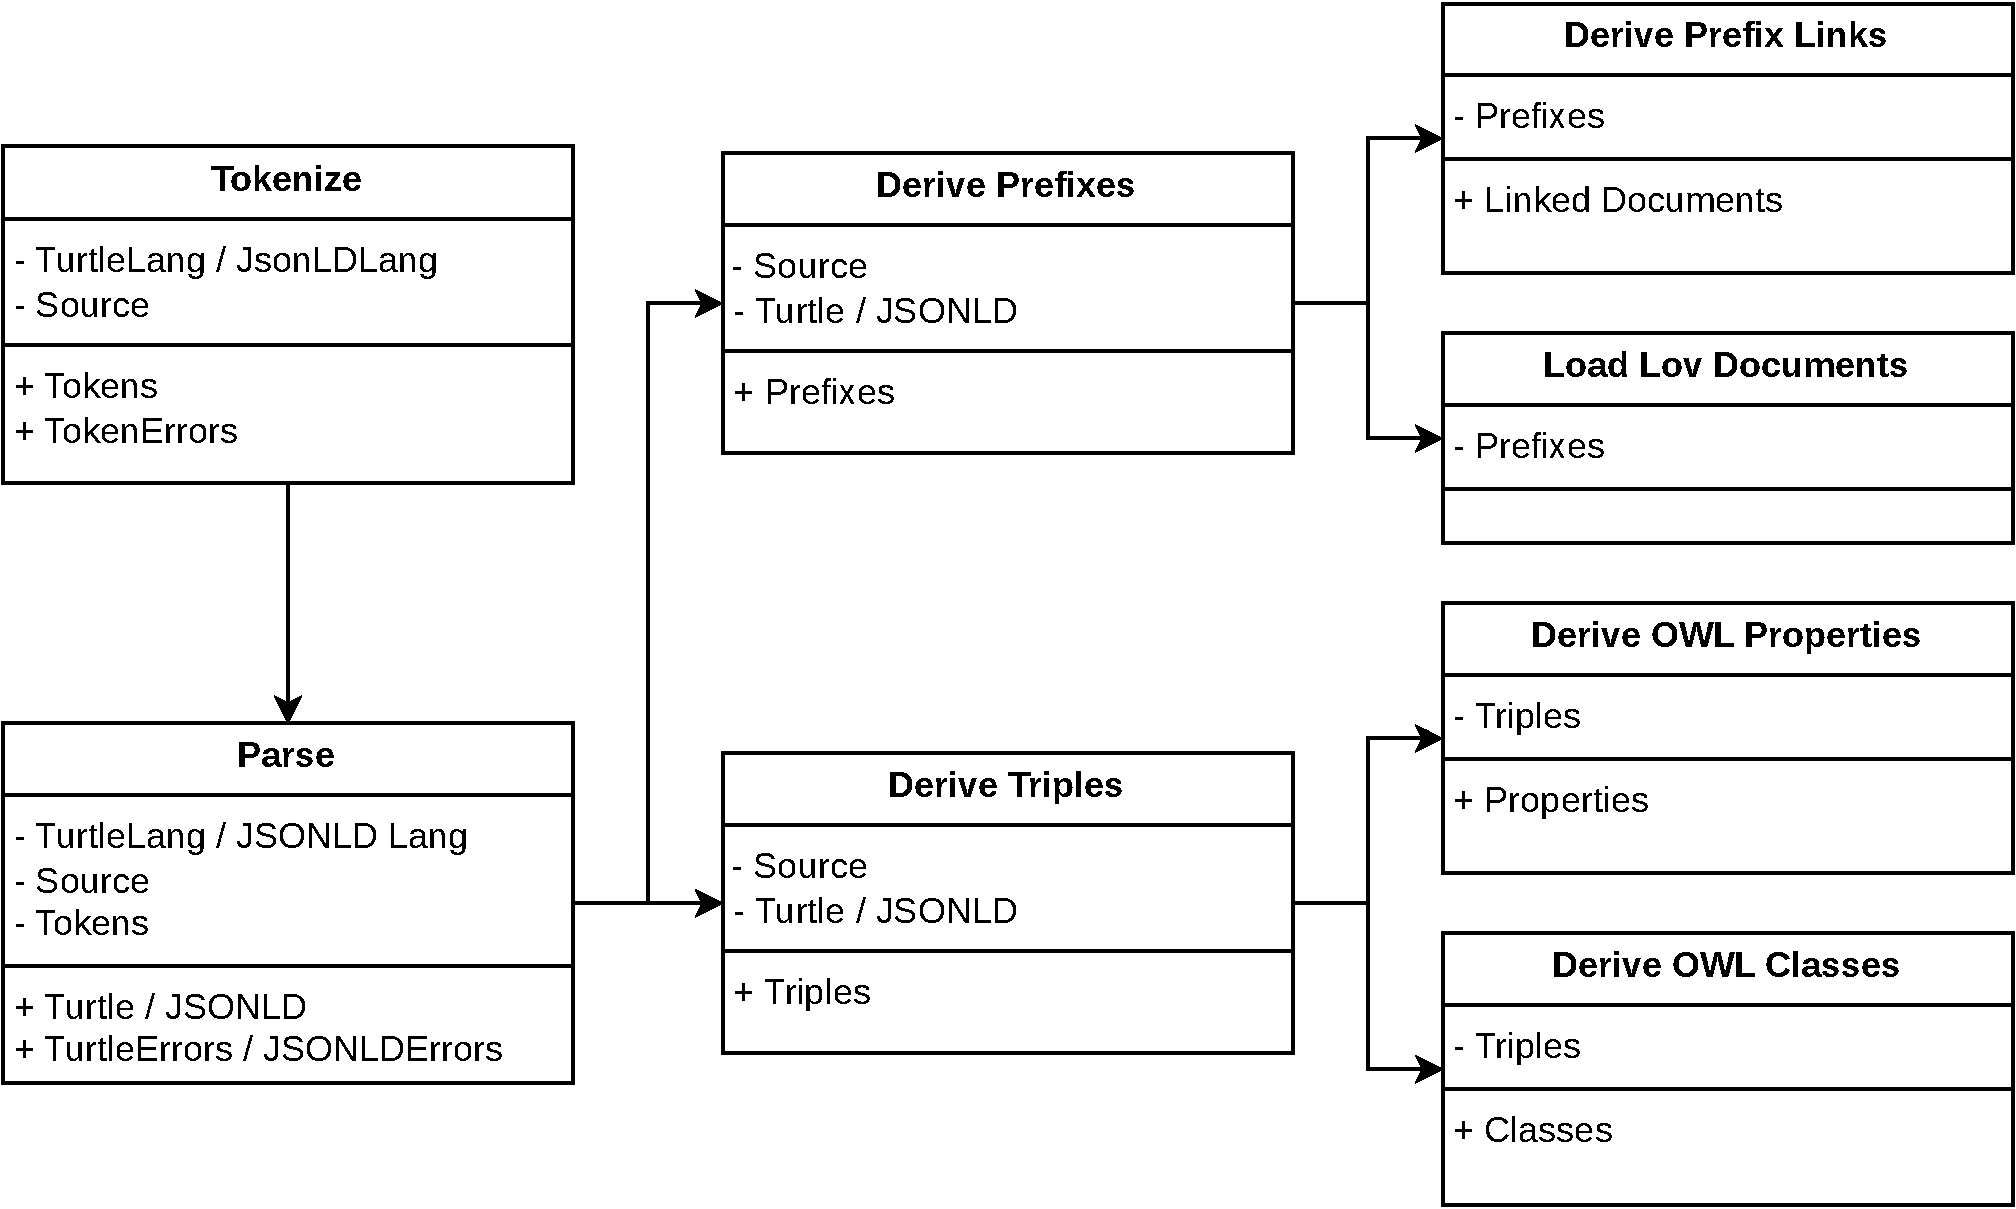
\includegraphics[width=1.2\textwidth]{./images/ParseSchedule.pdf}
 }
  \caption{Visual representation of the Parse schedule including tokenization, parsing, deriving prefixes, deriving triples, linking documents, fetching LOV documents, deriving properties and deriving classes. }\label{fig:Parse}
\end{figure}

The parsing schedule is one of the most important schedules of the language server.
It is activated whenever the user edits a document, the language server is notified with the textual changes.

We chose to let all semantic languages use the same \texttt{token} type, this allows for implementing token based systems only once.
Note that each semantic language does it's own tokenization, not allowing for SPARQL tokens inside Turtle documents.
In Figure \ref{fig:Parse}, \textit{tokenize} is the first sytem in the parsing schedule, this system is implemented for all supported semantic languages. \textit{Tokenize} also report on tokenization errors.

The next system is \textit{parsing}, also implemented for each semantic language, transforming the tokens into actual objects, and reporting on syntactic errors. 
When the objects are parsed, systems are issued that derive prefixes and triples. 
Prefixes contain information about how to expand and shorten iri's for the current document.
Deriving triples does not only derive actual triples, but in the case for SPARQL also bindings, which can be thought of as \textit{triples}.

After deriving prefixes, other systems will create a \texttt{LinkedDocuments} component, listing all documents that are linked some way to this document.
Prefixes are one way, but the object value of the triple \texttt{<> owl:imports <otherLocation>.}, also linkes that other document with the current document.
Prefixes are also used to load the correct LOV defined ontologies, setting up documents containing property and class definitions.

When the triples are derived, a system will derive properties and classes.
In most documents this will result in no properties or classes, but a document linked from LOV will contain many.
The power of the entity component system is that all documents are handled exactly the same.
This allows to cover a use case where a domain expert is writing the ontology and creating SPARQL queries to see how the ontology \textit{feels}, just by importing a local ontology file.

\paragraph{Some words on parsing}

With the language server protocol the server can specify wether or not it requires only the (minimal) changes or entire document every time.
Earlier versions of the semantic lsp required the entire document every time, because documents arae relatively small and reprasing the entire document brings an acceptable performance.
However, we noticed that this hampered the implementation, in turtle specifically there are patterns that cannot be parsed correctly and brings incorrect and frustrating feedback to the user, and partial parsing helps in this regard.
An example is shown in \ref{lst:GroupedListing}.
  The user at \ref{code1} types named node \texttt{<b>}, the language server should not be confused: triple \texttt{<c> <d> <e>} has nothing to do with named node \texttt{<b>}. The language server should suggest objects that fulfill the domain of predicate \texttt{<b>}. 
  The user at \ref{code2} types named node \texttt{<c>}, the language server should not be confused: the are two triples \texttt{<a> <b> <c>} and \texttt{<a> <d> <e>}, however tokenwise the documents are the same. Resulting in the language server suggesting a semi colon.
  
  The user at \ref{code3} just wrote a subject, invocing the subject completion defined in the next section. The language server might incorrect suggest to add a comma after \texttt{<c>} to build a syntactically correct document.
  The user at \ref{code4} is typing a predicate for the subject \texttt{<a>}, the language server might incorrectly parse the document as seen at \ref{code3}, where \texttt{<b>} is subject thus not invocing the property completion as explained in the next section.

  Adding partial parsing eliminates these issues as the language server understand which tokens are new and leaving the original interpretation of the surrounding tokens in touch.


\begin{figure}[tb]
    \centering
    % code1
    \begin{subfigure}{0.21\textwidth}
      \lstinputlisting{./code/option1.ttl}
      \caption{User types \texttt{<b>}}
      \label{code1}
    \end{subfigure}
    \hfill
    % code 2
    \begin{subfigure}{0.21\textwidth}
      \lstinputlisting{./code/option2.ttl}
      \caption{User types \texttt{<c>}}
      \label{code2}
    \end{subfigure}
    \hfill
    % code 3
    \begin{subfigure}{0.21\textwidth}
      \lstinputlisting{./code/option3.ttl}
      \caption{User types \texttt{<a>}}
      \label{code3}
    \end{subfigure}
    \hfill
    % code 4
    \begin{subfigure}{0.21\textwidth}
      \lstinputlisting{./code/option4.ttl}
      \caption{User types \texttt{<b>}}
      \label{code4}
    \end{subfigure}
    \caption{Different code samples showing that it is the indentation/intent of the user that dictates how tokens should be parsed. (a) and (b) show five terms that result in different triples. (c) and (d) show four terms, triples with subject \texttt{<a>} and \texttt{<b>} and both triples with subject \texttt{<a>} resulting in different semantics.    }\label{lst:GroupedListing}
\end{figure}



\subsubsection{Completion}

Completion is one of the most important features that actively interacts with the user.
In the Langauge Server Protocol, the langauge server is issed a completion event that contains the current location of the user.
The server should then answer with a list of completions, including the textual operations, a title and potentially some documentation.
It's the responsibility of the editor to sort and filter the completions and show the user the most relevant information.
How editors do this is not specified, which makes it difficult to create comprehensive testing suite.

\begin{figure}[!ht]
 \centering
 \makebox[\textwidth]{%
    \includegraphics[width=1.2\textwidth]{./images/Completion.pdf}
 }
  \caption{Visual representation of our example pipeline, 
      loading sensor data from The Things Network into a triple store}\label{fig:Completion}
\end{figure}

Figure \ref{fig:Completion} shows a schematic overview of the different systems in the completion schedule and their interactions.
First the server will create a \texttt{CompletionRequest} object, currently containing no completions.
Systems add their relevant completions to the request which is then returned to the user.

The location the user at the moment of the request is not enough information to derive comprehensive completions, 
the first systems will extract more information that is then used by the systems that create the actual completions.

\texttt{GetCurrentToken} expands the current location to the current token, then \texttt{GetCurrentTriple} tries to find the triple that this token corresponds to also indicating whether the user is typing a subject, predicate or object.
If \texttt{GetCurrentToken} fails, the entity lacks a TokenComponent and results in \texttt{GetCurrentTriple} not being issued.

The language server has enough information with only the current token to complete based on defined subjects with the \texttt{SubjectCompletion} system.
The server also completed on already defined prefixes (with \texttt{CompletePrefix}), this system is language agnostic as the Prefixes component is already defined.
To import new prefixes from LOV, each language has to implement a \texttt{CompleteLOVPrefix}, because how to add the import statement is language specific.


\subsubsection{Diagnostics}

The Diagnostics component of the Semantic Language Server (SLS) comprises several focused systems that analyze parsed data to identify issues and provide feedback to users.
Diagnostics differ fundamentally from other language server functionalities because they are push-based: the server actively notifies the editor of errors and warnings.
This allows for timely feedback, ensuring that users can quickly identify and address problems in their semantic documents.

Diagnostics are triggered with two different schedules: on edit and on save.

\begin{enumerate}
  \item \textit{On edit} diagnostics provide fast, real-time feedback to users, enabling them to fix errors as they type. 
    This ensures a fluid editing experience and minimizes interruptions.
  \item \textit{On save} diagnostics occur less frequently and are therefore better suited to more computationally intensive checks,
   such as validation against SHACL shapes.
\end{enumerate}

To demonstrate the capabilities of the diagnostics system, we highlight three key systems:

\begin{enumerate}
  \item \textit{Syntax Diagnostics:}
    During the tokenization and parsing phases, errors such as syntax mismatches or malformed input are detected and recorded, along with their locations.
    These errors are immediately passed to the diagnostics publisher resource, making this part of the on edit schedule, as the necessary data is already generated during parsing.
  \item \textit{SHACL Validation:} 
    With the on save schedule, the server uses the Rudof library to validate the current document against SHACL shapes.
    Shapes are dynamically extracted from the document itself, as well as from prefix links and owl:imports statements.
    This system ensures that the semantic data conforms to expected structural and logical constraints, enabling robust validation for ontologies and linked data documents.
  \item \textit{Basic Validation:}
    This system identifies common issues, such as undefined prefixes or unused declarations.
    By flagging such problems, it helps users maintain consistency and avoid errors that might lead to interoperability issues.
\end{enumerate}

Together, these systems provide comprehensive diagnostic support, catering to both immediate feedback needs and more in-depth validation processes.
This modular approach ensures that diagnostics remain lightweight yet powerful, accommodating the diverse requirements of semantic web practitioners.

\subsubsection{Varia}

Beyond core functionalities, the Semantic Language Server (SLS) offers additional schedules that enhance the user experience and round out its capabilities.
These schedules are smaller in scope, generally focusing on presentation or user interaction rather than deriving new information.

The most notable are as follows:
\begin{enumerate}
  \item \textit{Formatting:}
    A consistent document structure improves readability and reduces the cognitive load required to parse data visually.
    As a formatter, the language server ensures uniformity across documents, promoting best practices and easing collaboration.
    Currently, the SLS includes an opinionated formatter for Turtle, which automatically applies a standardized layout to documents.

  \item \textit{Hover:}
    Hover functionality provides contextual insights about symbols in the document, offering users additional information without disrupting their workflow,
    allowing for users to explore semantic relationships and documentation seamlessly.
    The SLS’s hover implementation includes three key features:
    \begin{itemize}
      \item Type Information: For a node with an inferred type, the hover popup displays the type alongside its hierarchy, including subclasses and superclasses.
      \item Class Details: Hovering over a class reveals its \texttt{rdfs:description}.
      \item Property Insights: Hovering over a property shows its \texttt{rdfs:description}, as well as its range and domain.
    \end{itemize}

  \item \textit{Highlighting:}
    Highlighting improves document readability by visually distinguishing between elements.
    The SLS implements both syntax highlighting and semantic highlighting through a two-step process:
        An initial system maps all tokens to their basic semantic types.
        Subsequent systems refine the types based on additional information.
    For example, in JSON-LD, all keys are initially highlighted as strings.
    However, keys starting with the \texttt{@} symbol are reclassified as keywords, enhancing clarity and usability for JSON-LD documents.
\end{enumerate}

These schedules, while smaller in scale, significantly enhance the language server’s utility by making semantic documents more intuitive and easier to work with.
They represent the \textit{polish} that transforms SLS into a complete tool for semantic web practitioners.
